\begin{exercises} 
\item Let $f$ be a function with the following properties:  $f$ is differentiable at every value of $x$ (that is, $f$ has a derivative at every point), $f(-2) = 1$, and $f'(-2) = -2$, $f'(-1) = -1$, $f'(0) = 0$, $f'(1) = 1$, and $f'(2) = 2$.
\ba
	\item On the axes provided at left in Figure~\ref{F:1.4.Ez1}, sketch a possible graph of $y = f(x)$.  Explain why your graph meets the stated criteria.
	\item On the axes at right in Figure~\ref{F:1.4.Ez1}, sketch a possible graph of $y = f'(x)$.  What type of curve does the provided data suggest for the graph of $y = f'(x)$?
	\item Conjecture a formula for the function $y = f(x)$.  Use the limit definition of the derivative to determine the corresponding formula for $y = f'(x)$.  Discuss both graphical and algebraic evidence for whether or not your conjecture is correct.
\ea
\begin{figure}[h]
  \begin{center}
 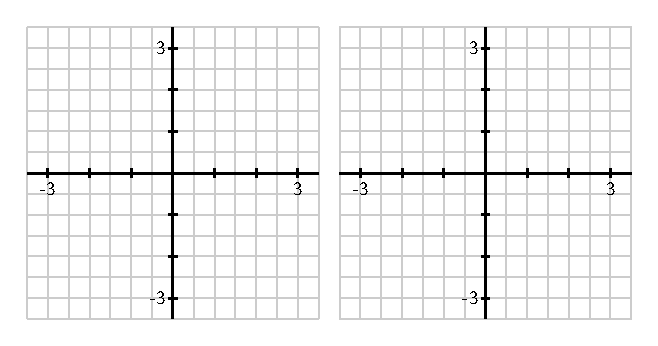
\includegraphics{figures/1_2_Ez3.eps} %\ \  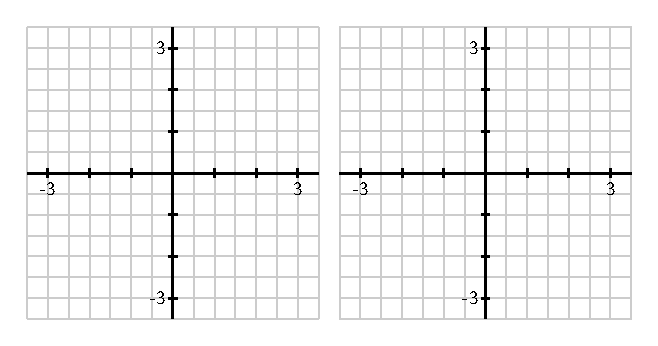
\includegraphics{figures/1_2_Ez3.eps}
   \end{center}
   \caption{Axes for plotting $y = f(x)$ in (a) and $y = f'(x)$ in (b).} \label{F:1.4.Ez1}
\end{figure}
\begin{exerciseSolution}
\end{exerciseSolution}

\item Consider the function $g(x) = x^2 - x + 3$.
\ba
	\item Use the limit definition of the derivative to determine a formula for $g'(x)$.
	\item Use a graphing utility to plot both $y = g(x)$ and your result for $y = g'(x)$; does your formula for $g'(x)$ generate the graph you expected?
	\item Use the limit definition of the derivative to find a formula for $h'(x)$ where $h(x) = 5x^2 - 4x + 12.$
	\item Compare and contrast the formulas for $g'(x)$ and $h'(x)$ you have found.  How do the constants 5, 4, 12, and 3 affect the results?
\ea	


\item Let $g$ be a continuous function (that is, one with no jumps or holes in the graph) and suppose that a graph of $y= g'(x)$ is given by the graph  on the right in Figure~\ref{F:1.4.Ez2}.
\begin{figure}[h]
  \begin{center}
 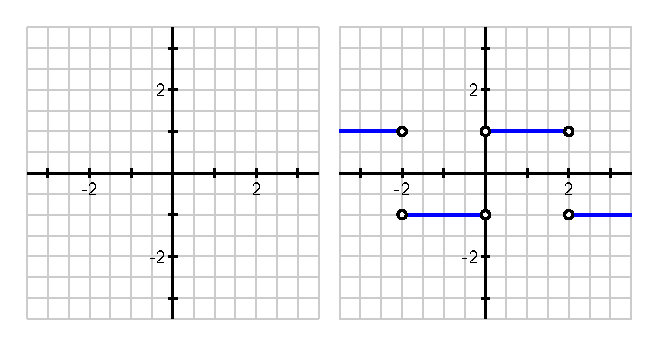
\includegraphics{figures/1_4_Ez2.eps} %\ \  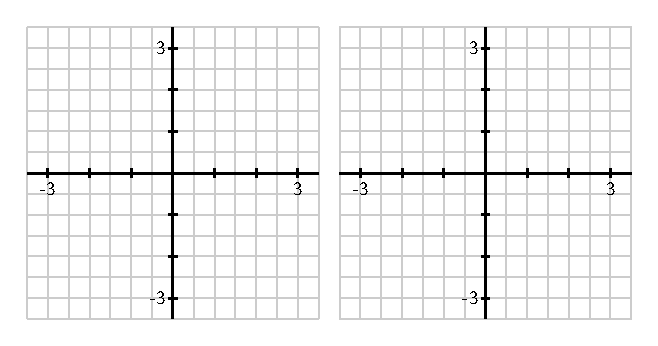
\includegraphics{figures/1_2_Ez3.eps}
   \end{center}
   \caption{Axes for plotting $y = g(x)$ and, at right, the graph of $y = g'(x)$.} \label{F:1.4.Ez2}
\end{figure}
\ba
	\item Observe that for every value of $x$ that satisfies $0 < x < 2$, the value of $g'(x)$ is constant.  What does this tell you about the behavior of the graph of $y = g(x)$ on this interval?
	\item On what intervals other than $0 < x < 2$ do you expect $y = g(x)$ to be a linear function?  Why?
	\item At which values of $x$ is $g'(x)$ not defined?  What behavior does this lead you to expect to see in the graph of $y=g(x)$?
	\item Suppose that $g(0) = 1$.  On the axes provided at left in  Figure~\ref{F:1.4.Ez2}, sketch an accurate graph of $y = g(x)$.
\ea

\newpage

\item For each graph that provides an original function $y = f(x)$ in Figure~\ref{F:1.4.Ez3a} (on the following page), your task is to sketch an approximate graph of its derivative function, $y = f'(x)$, on the axes immediately below.  View the scale of the grid for the graph of $f$ as being $1 \times 1$, and assume the horizontal scale of the grid for the graph of $f'$ is identical to that for $f$.  If you need to adjust the vertical scale on the axes for the graph of $f'$, you should label that accordingly.

\begin{figure}[h]
  \begin{center}
\scalebox{0.75}{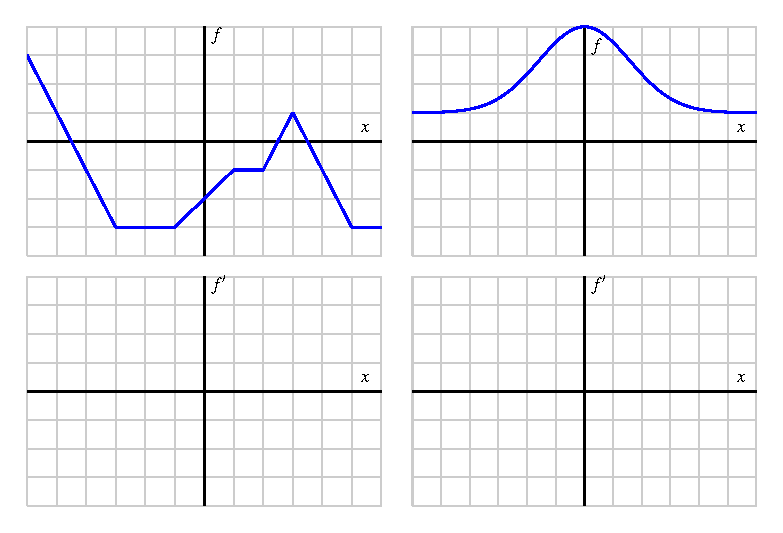
\includegraphics{figures/1_4_Ez3a.eps}} \\
\underline{\hspace{4in}}\\
\ \\
\scalebox{0.75}{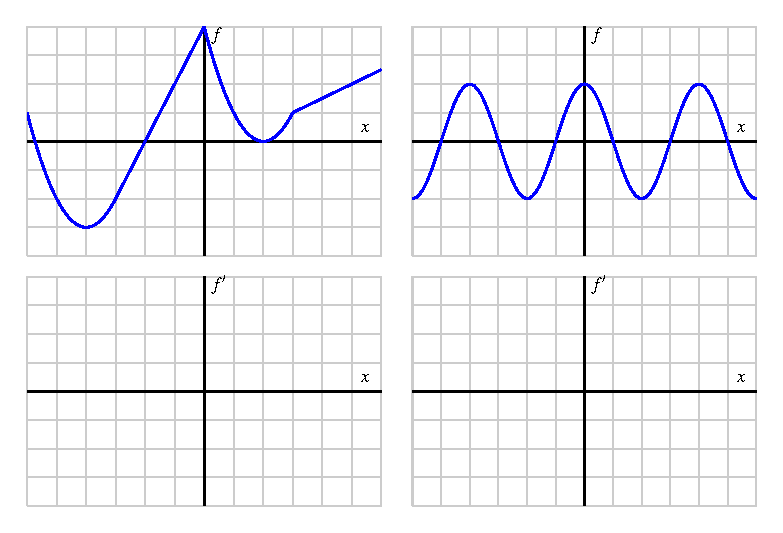
\includegraphics{figures/1_4_Ez3b.eps}}
   \end{center}
   \caption{Graphs of $y = f(x)$ and grids for plotting the corresponding graph of $y = f'(x)$.} \label{F:1.4.Ez3a}
\end{figure}







\end{exercises}
\afterexercises